\section{Driving Support Systems}

In this document we are mainly concerned about driving assistance. However, driving assistance is a vast research field with almost a century of evolution. Such systems aims to support the driver in the action of driving, this support is given in any form: visual alerts, auditory perception, actuators or haptics\cite{riener2010sensor}.

Since its appearance at the middle 50's, driving assistance has gained several branches, those branches have been heavily studied and currently are the target of many research centers.

Drive-support systems are becoming more and more popular. There exist several reasons, all of them mostly related with reducing \textbf{risk of incidents} and/or increasing the \textbf{confort} of driving. 

The former is linked with the cognitive overload in which the human is submited to. Off course the cognitive limitation is not an absolute number, it varies according to several parameters like mental health, type of the channel used (visual, auditory, tactile), amount of information transmitted, etc. A research conducted 2008 had the intend to study the human cognitive limitation for visual (eye) channel, basing this limitation in the saccadic movement of the eye and in the channel information capacity theorem\cite{LautarutisV}. The latter is linked to the anatomy of the instruments and the means used by the driver to perform an activity.

The human eye provides the largest amount of information for the brain. As the human visual sensors gives the major part of the world perception to the brain, it becomes per consequence the most used sensor.

The action of driving did not change since its creation, but the environment has. Due to this evolution the Advanced Driver Assistence Systems (ADAS) was coined to characterize advanced techniques that enhances the capability of driving, improving the vehicle-handling performance and at the same time reduce the workload for the driver\cite{riener2010sensor}.

The engineering of those types of systems is not related directly to computer science. The first mechanisms ever created for driving-support were purely mechanic, some examples of such systems are Cruise Control(CC), Anti-lock Break System (ABS), Collision Avoidance System(CAS).

\textbf{ADAS} is handled separately by researchers. Among the inumerous fields of application (Figure \ref{fig:sensor:target}), this work will concentrate in application situated in \textbf{Safety} branch.

\begin{figure}[h]
\centering
	\begin{tabular}{lr}\\
		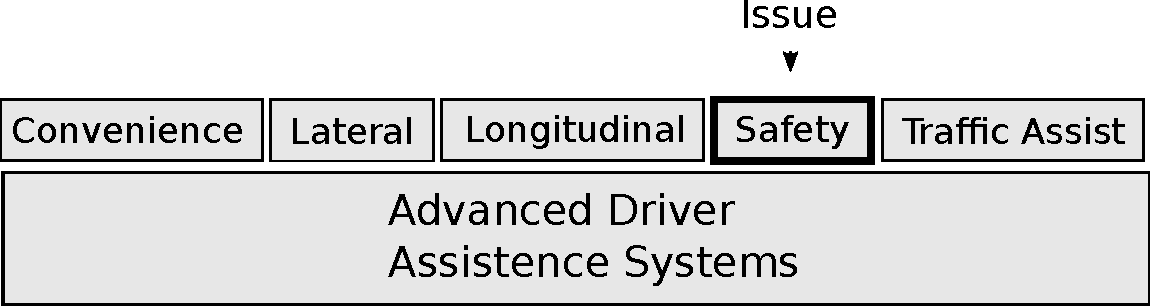
\includegraphics[scale=0.7]{img/fig:sensor:target} 
	\end{tabular}
	\caption{ADAS application stack and problem to be tacked (adapted from \cite{riener2010sensor})}
	\label{fig:sensor:target}
\end{figure}

Advanced Driver Assistence Systems must to perceive the environment before act. ADAS works just like the human cognition, it requires a mean to perceive the environment before dispatch any cognitive action. In the humanbody the environment perception is addressed by the eyes, although ADAS requires some artificial kind of sensing, that mimics the environment. 

The different ways of perceiving the environment and different types of technology used to achieve characterizes the sensing instruments, usually called \textbf{sensors}.

%% reviewed until here

In this paper we are concerned with electromagnetic radiation scanners, LIDAR(Light Detection and Ranging) laser for instance.

\subsection{Sensors}

%maybe replace the world system in the diagram and text by "control systems"

Pragmatically interacting with the physical environment requires sensing. Sensing is input for enumerous biological systems (e.g. nervous system, diggestive system), enabling such systems to respond properly to the changes observed by the sensors. 

\begin{figure}[h]
   \centering
     \begin{tabular}{lr}
       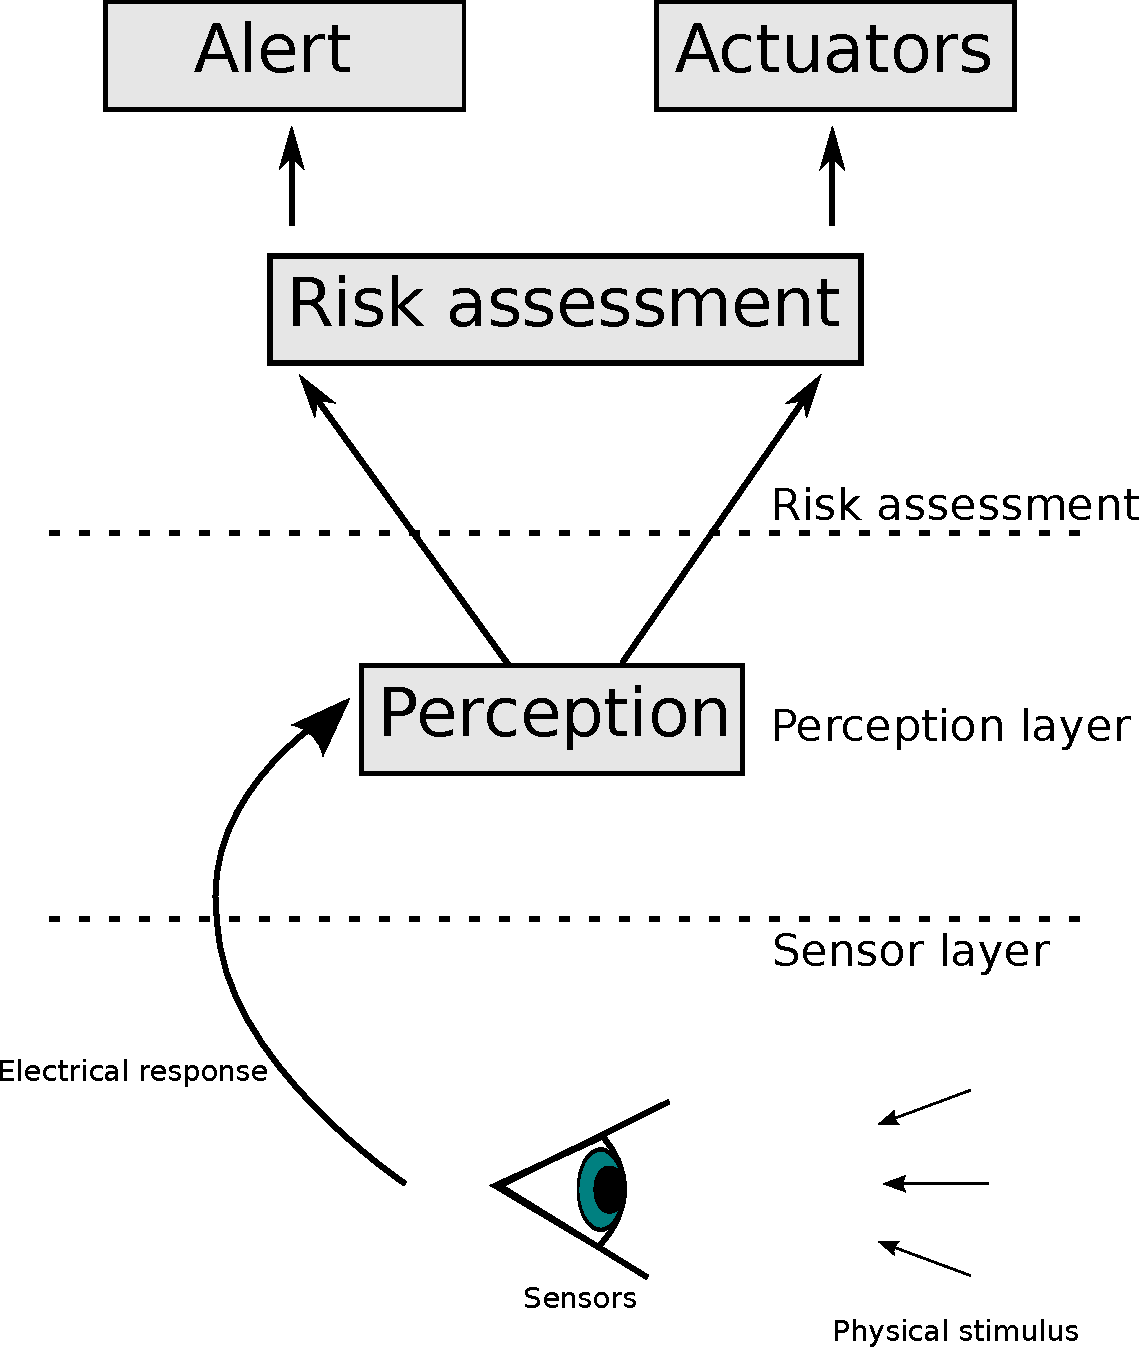
\includegraphics[scale=0.45]{img/fig:sensors:role}
     \end{tabular}
   \caption{The general architecture of a system attached to sensors}
   \label{fig:sensors:role}
 \end{figure}

Sensors do not perform action. They are the means in which complex systems acquire informations about the environment. Although, the sensors play a key role in almost every systems, they are located in a low laywer (Figure \ref{fig:sensors:role}), meaning that they have a low level of importance in terms of processing/filtering the data. Normally, incapable to responde direct to external stimulus without a system to observe the input data (provided by one or multiple sensors). The system react to the sensor stymulus through other means.

Thus, sensor is just responsible for the data aquisition (physical or electric) for a system located in a upper layer level of abstraction.

\subsubsection{Types}

There are virtually sensors for all kinds of properties (Figure\ref{fig:sensors}) that can be observed by sensors - in sometimes literatures called of \textbf{measurands}. They are essentially classified based in the measurands for which they were designed for.

\begin{figure}[h]
   \centering
     \begin{tabular}{lr}
       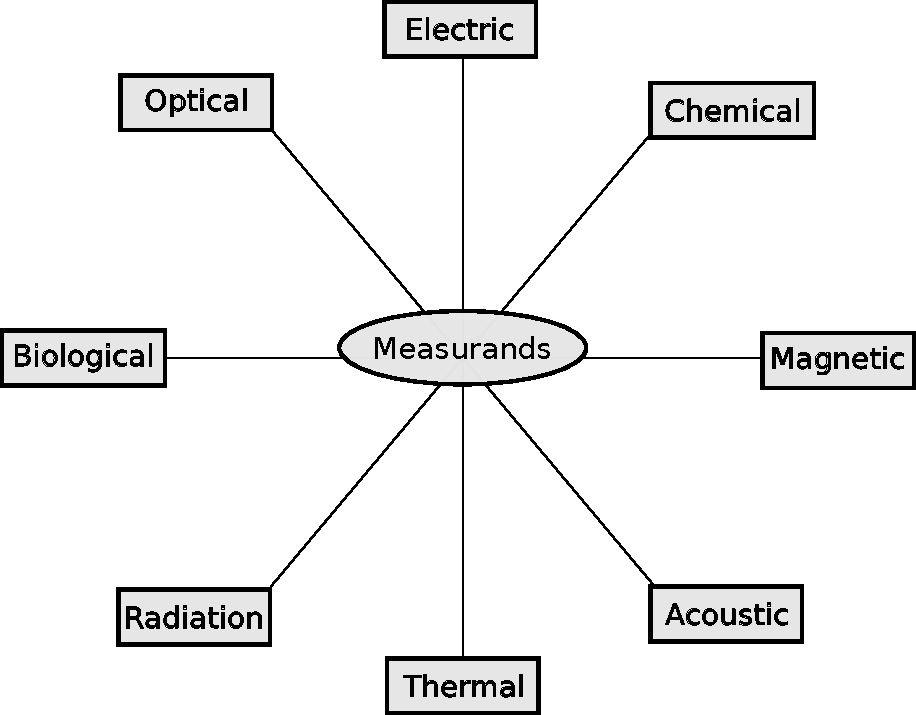
\includegraphics[scale=0.50]{img/fig:sensors}
     \end{tabular}
   \caption{Different types of measurands (adapted from \cite{WhiteRichard})}
   \label{fig:sensors}
 \end{figure}

\subsubsection{Properties}

The sensors are subject to issues. As the sensor is the capacity of a system to observe the environment, this affects diretly the solution (the main purpose of its existence).

The most common issues are: noise, imprecision. 

\paragraph{Noise} depending on the mean used by the sensor to perceive the physical events, it may become more of less subjected to interferances. Those interferances can cause instability in the data acquisition, possibly leading to its miss interpretations.

\paragraph{Imprecision} sensors rely on physical properties of the observed \textbf{measurands}, those properties may vary according to the environment in which the sensor is deployed.

Light Detection and Ranging can be a good example of imprecision. LIDARs uses light to measure the distance from objects, it does this by counting the time taken to the light hit the object and be reflected back. Although in the space the speed of the light is constant, in earth it depends on density of the atmosphere, amount of water particles in the air, among others. All those properties can change the speed of the light, thus, influencing dramatically the measurements.

\section{Perception}

Before talk about perception, its necessary to comprehend few concepts. Those concepts will frequently appear during this work: \textit{localization} and \textit{mapping}.

Localization provides the coordinnate of a point with respect to a static reference, this gives to this point a spatial positionning where an system actor (ego-robot) is using some reference which belongs statically to the environment.  

Mapping, as general knowledge, gives us information about a place, this representation gives as nothing but the static objects position. This might be confusion at some point, but this static objects positioning is provided using as reference other statics objects, and this is the key for this understanding.

By putting these two concepts together, we can go even further. Imagine the following situation, we have a map in our hands (provided by the environment \textit{mapping}) and we know exactly where we are in this map (by \textit{localization}), what would be the result of moving in this environment blind folded? Not good.

For the exactly same reason we need constantly to have the location of the moving object in the very same map, this is called \textit{tracking of moving objects} or even just \textit{tracking} \cite{Wang04a}.

In the next sessions we are going to see in more details the approaches utilized by robotics research to tackle the localization and mapping issues.

\subsection{SLAM}

SLAM (Simultaneous Localization and Mapping) is an approach that tries to solve concurrently the \textit{mapping} and \textit{localization} issues\cite{VU-2009-454238}. In this approach its assumed that the the initial position of the ego-robot is unknown. 

In such approach,  the observation acquired by the robot's sensor should be used. The sensor reading should be enough to obtain the robot's \textit{localization}. That localization coordinates (one or several in case of incertainties) must be visible in the current map of the environment. 

Although, this model requires a precise \textit{mapping} of the environment. This precision is required duo to parallel actions performed by the robot: moving itself in the (which change the enviroment from the robots perspective) and localizing the robot at the same time, and as the robot motion is performed in a continuous space, any interference in the measurements are accumulated and can affect severely the localization, diverging the calculated position from the real position.

The robot actions are subject of physical interferances as well. Depending in the kind of terrain in which the robot is moving affects how the robot movements can be trusted \cite{DBLP:conf/icra/LenainTHM11}. 

Thus, \textbf{inertia} plays a key role in the trustability of the robot movements. Other properties affects \textbf{inertia} such as: balance, weight distribution, grip condition, type of movement, etc.

All those variations bring an imprecision factor into the movement performed by a robot. This because those properties determines the resistence of the robot in changing its speed.

From the probabilist point of view, this implies in estimate the joint probability distribution (Equation \ref{jpd:discrete}). Where the $u$ represents the observations and $z$ the measurements.

Thus, the output of the SLAM process is the robot pose and a map of the stationary objects captured by the \textit{perception} sensors \cite{iyengar1991autonomous}.

\subsubsection{Formalization}

In SLAM, our main concern is to localize ourselves and the static objects in the surrouding environment. 

Intending to simplify the perspective of this problem, we will generate a scenario that will be used in analogy to the formula and may help the reader to absorbe the intuition behind the formalization.

\paragraph*{Lost Robot} is positioned arbitrarily in a finite space unknown. This is a classical 4 wheeled robot. This same robot is subject of any kind of random forces and terrain condition. 

Suppose we send a command to the robot to move one centimeter ahead, how do we ensure that he really changed one centimeter? Suppose that without observing the last position of the robot we send another command to move another centimeter ahead. 

Thus, everytime we actuate in the robot without checking the real position, the incertainty grows, and the possible new position increases exponentially.

Formalization of such dependency can be done through \textit{Bayes rule}. Bayes rule define the \textit{posteriori} probability distribution over a set $X$, normally represented as $p(A | B)$, which can be read as probability of $A$ knowing $B$.

\begin{equation}
\label{jpd:discrete}
P(x_t,M | z_{0:t}, u_{1:t})
\end{equation}


\subsection{DATMO}

Detection and Tracking of Moving Objects (DATMO) was initially studied by radar tracking systems \cite{VU-2009-454238} researches. Since in RADAR only moving objects are visible.

Those objects in scene they must solve the data association problem. The former assumption is unrealistic in the vision of a robot, the perception sensor senses all objects, independently on their motion, so static and dynamic objects are included in the representation.

As DATMO is a large process, some researchers chose to pick just a part of this process, which is "Moving Object Tracking" and solve it, without worry about the detection phase.

DATMO responsability is to:

\begin{itemize}
\item Detect and initialize new objects
\item Remove objects that went out of the scene
\item Moving object motion modeling
\item Data association
\end{itemize}



\subsection{SLAMMOT}

Researches considered SLAM and DATMO as two different problems that should be solved separately, \textit{Wang} was one of the first researches to put in evidence the similarities between both problems \cite{Wang03onlinesimultaneous}.

As result, the SLAMMOT term was coined and a derivation of the SLAM formula with DATMO was created to simplify the process of tracking. The experiment showed that solving the SLAM with DATMO increased dramatically the performance of the algorithm comparing them with the results as individual solutions (performance was verified in crowded urban environment).

\begin{figure}[h]
   \centering
     \begin{tabular}{lr}
       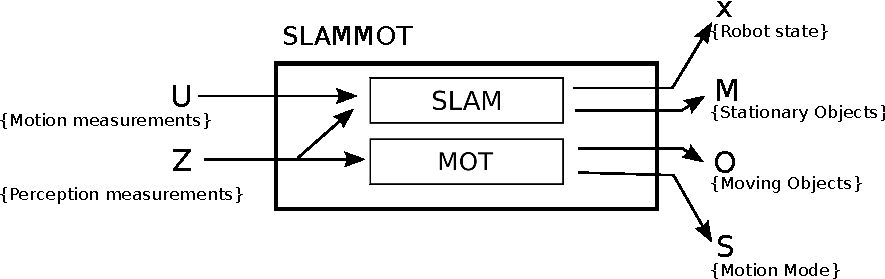
\includegraphics[scale=0.9]{img/fig:slammot}
     \end{tabular}
   \caption{SLAMMOT composition (adapted from \cite{Wang04a})}
   \label{fig:slammot}
 \end{figure}

As the GPS system or an good IMU for a good precision are too expensive, the paper propose a bayesian approach solution which satisties the navigation constraints without compromise the safety and at the sametime are not high costly as the other solutions based on a specialized hardware.

\subsection{SLAM and DATMO}

Robots face a set of problems which are common among many robots, how to move in a certain environment is one of them.

The general environment perception (Figure \ref{fig:perception:cycle}) requires at least two inputs: the perception measurements $Z$ which are usually are provided by cameras, LIDAR, or even radars, and motion measurements provided by the IMU (Inertial Measurement Unit).

\begin{figure}[h]
   \centering
     \begin{tabular}{lr}
       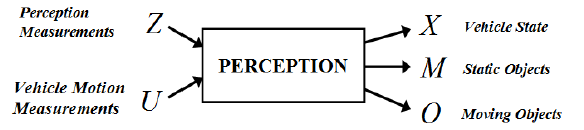
\includegraphics[scale=0.5]{img/fig:perception:cycle}
     \end{tabular}
   \caption{Perception cycle}
   \label{fig:perception:cycle}
 \end{figure}


He perceives the environment by using as input sensors informations and can be composed of several sensors, or even heterogeneous types of sensors, and those give a partial observation of the environment (according with the current technology applied in those sensors). Thus, the robot does not known what paths can be perceived to reach a given point in a space.

So, knowing the positions that can be assumed by the robot is essential and necessary so robot cat move in this environment, this is done by observing the environment through the sensors and creating a spatial relation between the static objects in this space, this is known as SLAM - or Simultaneous Localizations and Mapping \cite{iyengar1991autonomous}.

Although, this just concern a small set of the problems related with robots applications, for instance robots that are used for mining, in this type of environment the only element that can change the environment and the spatial relation between the static objects is the robot itself. 

Depending in the goal of the robots perception, may be required to make distinction between each object, with cameras we can use characteristics like color, shape. Whereas, classify an object based in a LIDAR or radar information neither shape nor color are available, at least not directly without pre-processing.

Another set of problems concerns the most part of robots applications are highly dynamic environments, where the objects can change their position with respect to the static environment, those objects can become an obstacle for the robots, for this reason its necessary to map those objects, this relation called DATMO - Detection and Tracking of Moving Objects.

Although these two classification are given in a separate manner, they can be used as complementary to each other as presented in the paper \cite{Wang04a}, which will be dissected later.

\subsection{Spatial representation}

There exists several ways to represent one environment in with respect to its spatial information. Occupancy Grid is one of these methods and it is largely applied, its built based on a multidimensional field that maintains the occupancy state information in a cell\cite{Elfes:1989:UOG:68491.68495}. Those cells are built in a regular size, and the number of cells which compose the grid is algorithm dependent.

At the same time Occupancy Grid (a.k.a. certainty grids) is effective in data representation it is also effective in represent sensor fusion information with it. Occupancy grid can be used as well to represent tree-dimentional environment, as was demonstrated in a small submersible craft, that looks for old battleships in the bottom of the ocean\cite{DBLP:journals/aim/Moravec88}.

One variation of the occupancy filter - The Bayesian Occupancy Filter(BOF) - contains the velocity and the probability distribution in Bayesian framework.

\subsection{Occupancy grid mapping}

Representing continous space when dealing with the uncertainty of an action of a mobile robot is extremely demanding in terms of resource usage, either in terms of processing power or memory allocation.

Thus, targeting to amortize the computational requirement for the incertainty in the displacement of a robot, discretization models are used, Occupancy Grid\cite{Elfes:1989:UOG:68491.68495} is one of the former models proposed to tackle this issue.

This kind of representations is done with multi-dimensional vectors and results in a bird-eye view of the discretized map obtained by the perception sensor Figure \ref{fig:grid:continuous:discretized}.


\begin{figure}[h]
\centering
	\begin{tabular}{lr}\\
		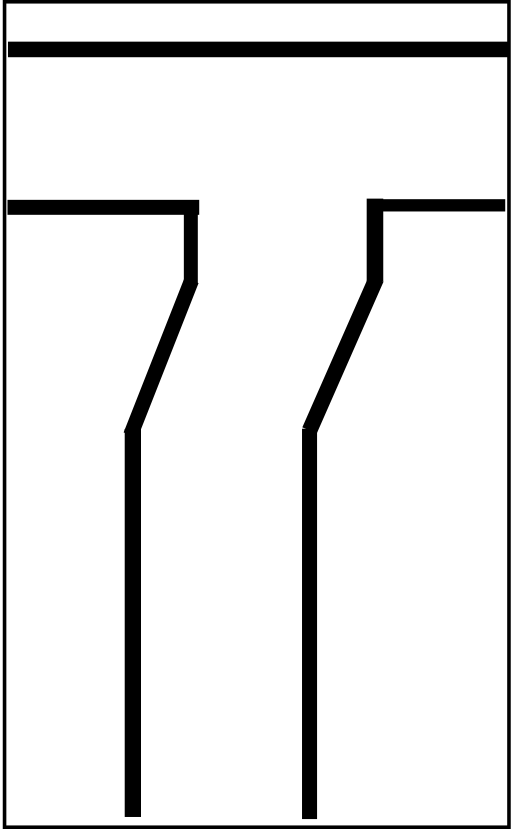
\includegraphics[width=0.25\columnwidth]{img/fig:grid:continuous} &
		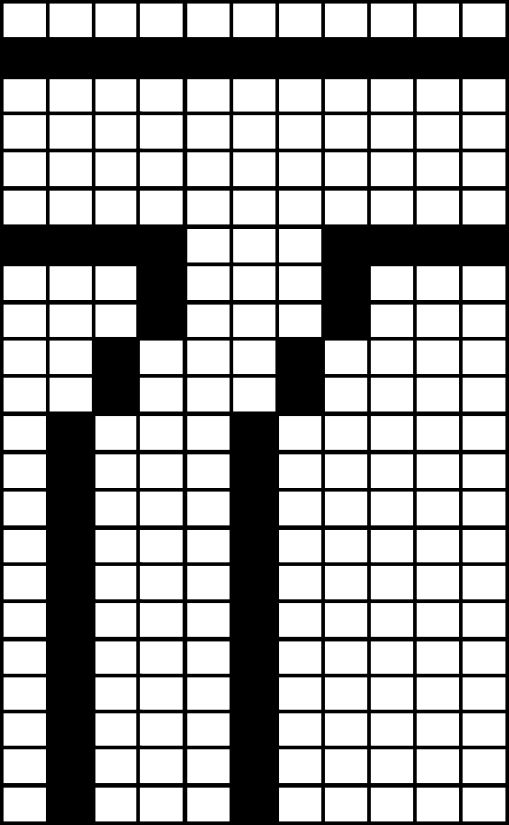
\includegraphics[width=0.25\columnwidth]{img/fig:grid:discretized}
	\end{tabular}
	\caption{Continuous \& discretized representation of a map}
	\label{fig:grid:continuous:discretized}
\end{figure}


In grid framework each cell $C$ can be assigned have its state $\phi(C)$ configured to binary domain, so, either the current state of the cell is \textit{occupied} or it is \textit{free}, in this paper we state that the value $1$ represents the occupied state and $0$ a $free$ space Equation \ref{eq:binarycell}.

\begin{equation}
P(\phi(C)=1) + P(\phi(C)=0) = 1
\label{eq:binarycell}
\end{equation}

This model can be extended to a more general model coined as \textit{inference grids} that encapsulate multiple properties\cite{Elfes:1989:OGP:916528}.

\textit{Goal: Why occupancy grid? how its built? }

\subsection{Object Separation}

\textit{Goal: u-disparity, uv-disparity}

\paragraph*{UV-disparity} 

UV disparity come off from an technique called U-disparity, a technique which aimed to separate the objects from the road surface.. (uv disparity slide 2)


\subsection{Classification}

\textit{Goal: talk about multimodels, importance sampling (or other statistical sampling method), prior map knowledge }

%multimodels, importance sampling, prior map knowledge

\section{Risk assessment}


